% Build: cd docs/reports/reconstruction/momentum_reco/ms_ablation && latexmk -xelatex ms_ablation_mixed_20260422.tex
\documentclass[a4paper, 11pt]{article}

\usepackage[margin=2.4cm]{geometry}
\usepackage{amsmath,amssymb}
\usepackage{booktabs}
\usepackage{array}
\usepackage{siunitx}
\usepackage{xcolor}
\usepackage{hyperref}
\usepackage{enumitem}
\usepackage{float}
\usepackage{graphicx}
\usepackage{caption}
\usepackage{subcaption}

\definecolor{airorange}{RGB}{230,140,40}
\definecolor{vacblue}{RGB}{30,90,180}

\hypersetup{
  colorlinks=true,
  linkcolor=blue!60!black,
  urlcolor=blue!60!black,
}

\newcommand{\air}{\textcolor{airorange}{\textbf{air}}}
\newcommand{\vac}{\textcolor{vacblue}{\textbf{vacuum}}}

\title{\textbf{PDC Multiple-Scattering Ablation:\\ Two-Region Geometry, Three Configurations}}
\author{Baiting Tian \\ RIKEN Nishina Center / DPOL Experiment}
\date{2026-04-22 (rev2)}

\begin{document}
\maketitle

\begin{abstract}
\noindent
This memo records three Geant4 ablation configurations of the SAMURAI~+~PDC setup that vary the vacuum/air distribution along the proton flight path, in order to quantify the air contribution to the PDC hit-position resolution $\sigma_y(\mathrm{PDC2})$. The target sits inside the dipole yoke cavity (yoke-local coordinate $z = -920$~mm, well inside the $\pm 1750$~mm cavity); the magnet cavity and the \texttt{VacuumDownstream} beam pipe are physically connected and share a single \texttt{BeamLineVacuum} switch. The flight path is partitioned into \textbf{two regions}: Region~A = magnet cavity + downstream pipe (target $\to$ ExitWindow, $\sim 4.3$~m), Region~B = ExitWindow $\to$ PDC1 $\to$ PDC2 ($\sim 2.0$~m). The three configurations give $\sigma_y(\mathrm{PDC2})$ of 12.8--14.9~mm (all-air), 6.8--8.2~mm (Region~B air only) and 0.95--1.00~mm (all-vacuum). The Region~B air contributes $\sigma_B = 6.7$--$8.2$~mm in quadrature (3-truth-point mean $\approx 7.4$~mm); the Region~A air contributes $\sigma_A = 9.8$--$12.9$~mm (mean $\approx 11.2$~mm).
\end{abstract}

\tableofcontents

% ============================================================
\section{Geometry and flight path}
% ============================================================

\subsection{Where the target sits}

The target centre (tree-gun injection point) is at world coordinates $(-12.5, 0.0, -1069.5)$~mm, tilted by $3^\circ$. After the yoke is rotated by $-30^\circ$ about the $Y$ axis, the target's \textbf{yoke-local coordinates} are $(-545.5, 0, -919.9)$~mm. The yoke's inner cavity (\texttt{vchamber\_cavity}) is a $\pm 1620 \times \pm 400 \times \pm 1750$~mm rectangular box plus a downstream trapezoidal extension. Since $z = -919.9$~mm lies inside $[-1750, +1750]$~mm, the target shares a single connected gas/vacuum volume with the magnet cavity.

\subsection{The two regions}

A particle leaving the target only crosses two materially controllable regions before reaching PDC2:

\begin{table}[H]
\centering
\caption{Two-region geometry. Lengths use the straight-line approximation (curvature corrections are second-order and ignored).}
\label{tab:path}
\begin{tabular}{clrl}
\toprule
\# & Physical volume & Length & Switch \\
\midrule
A & Magnet cavity \texttt{vchamber\_cavity} + \texttt{VacuumDownstream} pipe & $\sim 4.3$~m & \texttt{/samurai/geometry/BeamLineVacuum} \\
B & ExitWindow $\to$ PDC1 $\to$ PDC2 (free flight in world volume) & $\sim 2.0$~m & \texttt{/samurai/geometry/FillAir}  \\
\bottomrule
\end{tabular}
\end{table}

In Region~A, the straight-line distance from the target to the yoke cavity exit face (yoke-local $z = +1750$~mm) along the local $z$ axis is about 2.67~m (the proton is bent by $\sim 30^\circ$ in the 1.15~T field; arc-length minus straight-line is well under 10\%); the pipe segment from the yoke exit to the ExitWindow adds another $\sim 1.6$~m, totalling $\sim 4.3$~m. In Region~B, ExitWindow $\to$ PDC1 is about 0.97~m and PDC1 $\to$ PDC2 is 1.00~m.

\subsection{Physical connectivity}

The upstream flange of the \texttt{VacuumDownstream} pipe attaches to the yoke exit, so geometrically they form a single connected vessel; in code, both volumes' material is selected by the same \texttt{BeamLineVacuum} switch: \texttt{true} $\to$ \texttt{G4\_Galactic} (vacuum), \texttt{false} $\to$ world material (driven by \texttt{FillAir}). This is the principal correction in rev2 over stage~A$'$, where the pipe was hard-coded as vacuum and decoupled from the magnet cavity --- a configuration that is not physically realisable.

\subsection{Things to underline}

\begin{itemize}[nosep]
  \item \textbf{Real-experiment configuration is undecided}: whether Region~A is air or vacuum in the actual experiment is still under exploration; the three configurations here are simulation ablations, not statements about the planned experimental setup.
  \item \textbf{Target disabled}: all three configurations use \texttt{SetTarget false} (tree-gun injection); the target volume itself does not contribute to MS. The material around the target is whatever \texttt{vchamber\_cavity} contains.
\end{itemize}

% ============================================================
\section{The three test configurations}
% ============================================================

\begin{table}[H]
\centering
\caption{The three test configurations. \air = air (\texttt{G4\_AIR}); \vac = vacuum (\texttt{G4\_Galactic}).}
\label{tab:conditions}
\begin{tabular}{lcc}
\toprule
Configuration & Region~A (cavity + pipe) & Region~B (EW $\to$ PDCs) \\
\midrule
\textbf{all\_air}          & \air & \air \\
\textbf{beamline\_vacuum}  & \vac & \air \\
\textbf{all\_vacuum}       & \vac & \vac \\
\bottomrule
\end{tabular}
\end{table}

Geant4 macros (all under \verb|configs/simulation/DbeamTest/detailMag1to1.2T/|):

\begin{center}
\begin{tabular}{ll}
\toprule
Configuration & Key switches \\
\midrule
\texttt{all\_air}         & \verb|FillAir true| \\
\texttt{beamline\_vacuum} & \verb|FillAir true|\ \ +\ \ \verb|BeamLineVacuum true| \\
\texttt{all\_vacuum}      & \verb|FillAir false| \\
\bottomrule
\end{tabular}
\end{center}

\texttt{BeamLineVacuum} is independent of \texttt{FillAir}: as long as \texttt{BeamLineVacuum=true}, Region~A is vacuum, regardless of \texttt{FillAir}. \texttt{all\_vacuum} sets \texttt{FillAir=false} so the world volume is also vacuum, and Region~A then follows the world material (also vacuum) without any explicit \texttt{BeamLineVacuum} setting.

\subsection{Code controls}

\begin{enumerate}[nosep]
  \item \textbf{\texttt{DipoleConstruction::ConstructSub}}: the yoke inner cavity (\texttt{vchamber\_box} $\cup$ \texttt{vchamber\_trap}) is built as its own \texttt{G4LogicalVolume} \texttt{vchamber\_cavity\_log}; with \texttt{fBeamLineVacuum=true} its material is \texttt{G4\_Galactic}, otherwise the world material.
  \item \textbf{\texttt{VacuumDownstreamConstruction::ConstructSub}} (\emph{the rev2 change}): the pipe material is also selected by \texttt{fBeamLineVacuum}: \texttt{true} $\to$ \texttt{G4\_Galactic}, \texttt{false} $\to$ world material.
  \item \textbf{\texttt{DeutDetectorConstruction::Construct}}: calls \verb|SetBeamLineVacuum(fBeamLineVacuum)| before instantiating \texttt{VacuumDownstream}; passes the same flag to \texttt{DipoleConstruction}.
\end{enumerate}

% ============================================================
\section{Configuration and execution}
% ============================================================

\begin{center}
\begin{tabular}{ll}
\toprule
Item & Value \\
\midrule
ENSEMBLE\_SIZE              & 50 events per (truth point $\times$ configuration) \\
Seeds                       & SEED\_A=20260421, SEED\_B=20260422 (shared across configurations) \\
Truth points                & $(p_x, p_y)$ = $(0,0)$, $(100,0)$, $(0,20)$ MeV/$c$ \\
Particle                    & proton, $|\vec p|=627$~MeV/$c$, $\beta c p = 348.4$~MeV \\
Target                      & \texttt{SetTarget false} (tree-gun injection) \\
Reco                        & \verb|test_pdc_target_momentum_e2e --backend rk| \\
                            & \verb|--rk-fit-mode fixed-target-pdc-only| \\
$\sigma$ definition         & robust half-width $(p_{84}-p_{16})/2$ \\
\bottomrule
\end{tabular}
\end{center}

\begin{verbatim}
cd /home/tian/workspace/dpol/smsimulator5.5
bash scripts/analysis/ms_ablation/run_ablation.sh
\end{verbatim}

Outputs land in \verb|build/test_output/ms_ablation_air/|: one \texttt{dispersion\_summary.csv} per configuration subdirectory plus a top-level \texttt{compare.csv} and three overlay PNGs.

% ============================================================
\section{Per-configuration $\sigma$ results}
% ============================================================

\begin{table}[H]
\centering
\caption{PDC hit robust half-width $\sigma$ (mm) and PDC1$\to$PDC2 slope dispersion $\sigma_\theta$ (mrad). $\sigma_y(\mathrm{PDC2})$ in bold.}
\label{tab:sigma_raw}
\small
\begin{tabular}{lrrrrrrrr}
\toprule
Config & $p_x$ & $p_y$ & $\sigma_x(\mathrm{P1})$ & $\sigma_y(\mathrm{P1})$ & $\sigma_x(\mathrm{P2})$ & $\sigma_y(\mathrm{P2})$ & $\sigma_{\theta_x}$ & $\sigma_{\theta_y}$\\
\midrule
\texttt{all\_air}         & 0    & 0  & 3.071 &  9.736 & 3.669 & \textbf{12.826} & 12.279 & 9.240 \\
\texttt{all\_air}         & 100  & 0  & 3.838 & 10.492 & 5.377 & \textbf{12.751} & 15.768 & 8.277 \\
\texttt{all\_air}         & 0    & 20 & 3.372 & 13.039 & 4.065 & \textbf{14.927} & 21.709 & 7.846 \\
\addlinespace
\texttt{beamline\_vacuum} & 0    & 0  & 1.528 &  4.061 & 2.086 & \textbf{ 6.801} & 11.834 & 5.910 \\
\texttt{beamline\_vacuum} & 100  & 0  & 2.067 &  4.888 & 3.060 & \textbf{ 8.211} &  8.100 & 5.786 \\
\texttt{beamline\_vacuum} & 0    & 20 & 1.667 &  4.789 & 2.363 & \textbf{ 7.459} & 14.289 & 5.421 \\
\addlinespace
\texttt{all\_vacuum}      & 0    & 0  & 0.147 &  0.515 & 0.447 & \textbf{ 0.947} &  6.798 & 2.558 \\
\texttt{all\_vacuum}      & 100  & 0  & 0.154 &  0.364 & 0.416 & \textbf{ 0.999} &  4.075 & 1.956 \\
\texttt{all\_vacuum}      & 0    & 20 & 0.174 &  0.411 & 0.396 & \textbf{ 1.002} &  6.913 & 2.299 \\
\bottomrule
\end{tabular}
\end{table}

Across all three truth points every position $\sigma$ obeys \texttt{all\_air} $>$ \texttt{beamline\_vacuum} $>$ \texttt{all\_vacuum}, consistent with the physical expectation ``more air, more MS''. Overlay scatter plots in Figure~\ref{fig:overlays}.

\begin{figure}[H]
\centering
\begin{subfigure}{0.32\textwidth}
  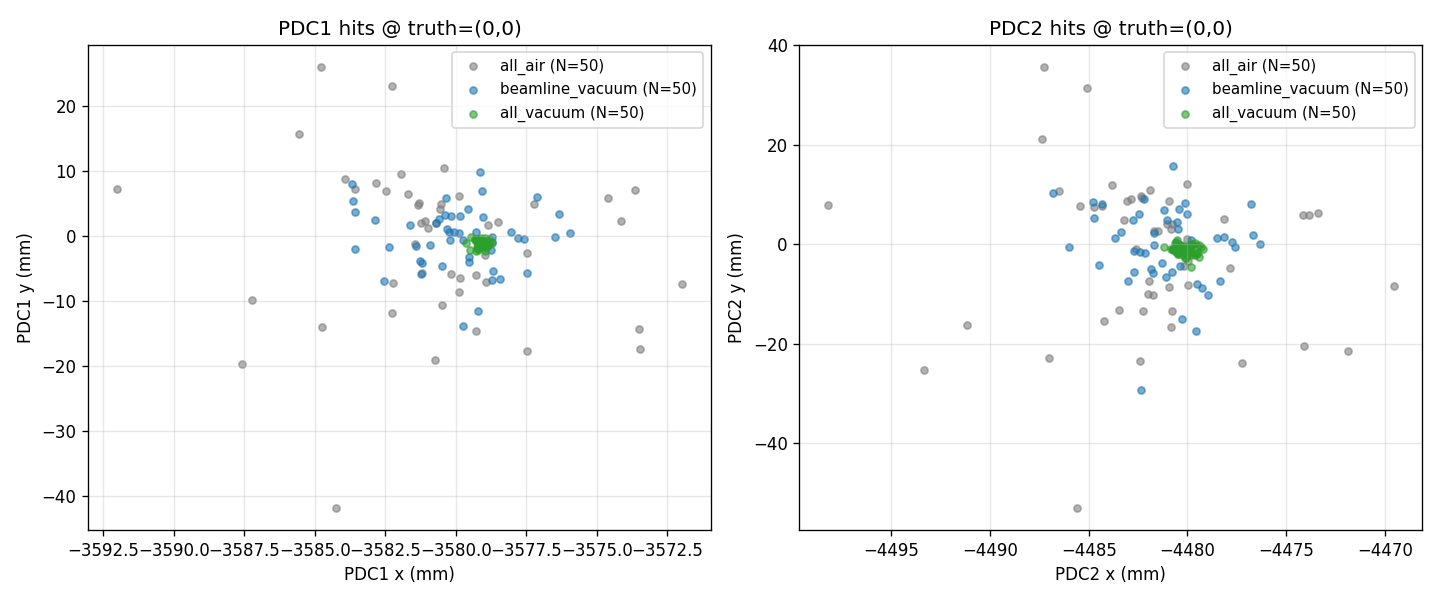
\includegraphics[width=\linewidth]{figures/dispersion_overlay_tp0_0.png}
  \caption{TP1: $(p_x,p_y)=(0,0)$}
\end{subfigure}
\hfill
\begin{subfigure}{0.32\textwidth}
  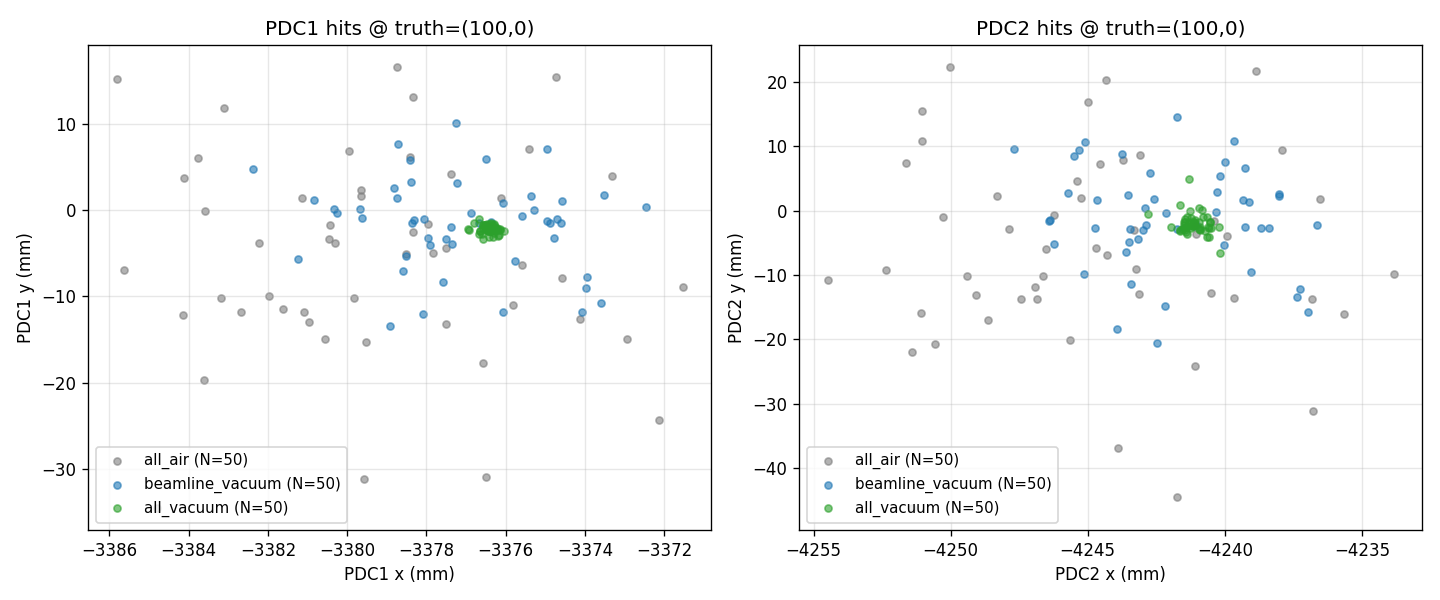
\includegraphics[width=\linewidth]{figures/dispersion_overlay_tp100_0.png}
  \caption{TP2: $(p_x,p_y)=(100,0)$}
\end{subfigure}
\hfill
\begin{subfigure}{0.32\textwidth}
  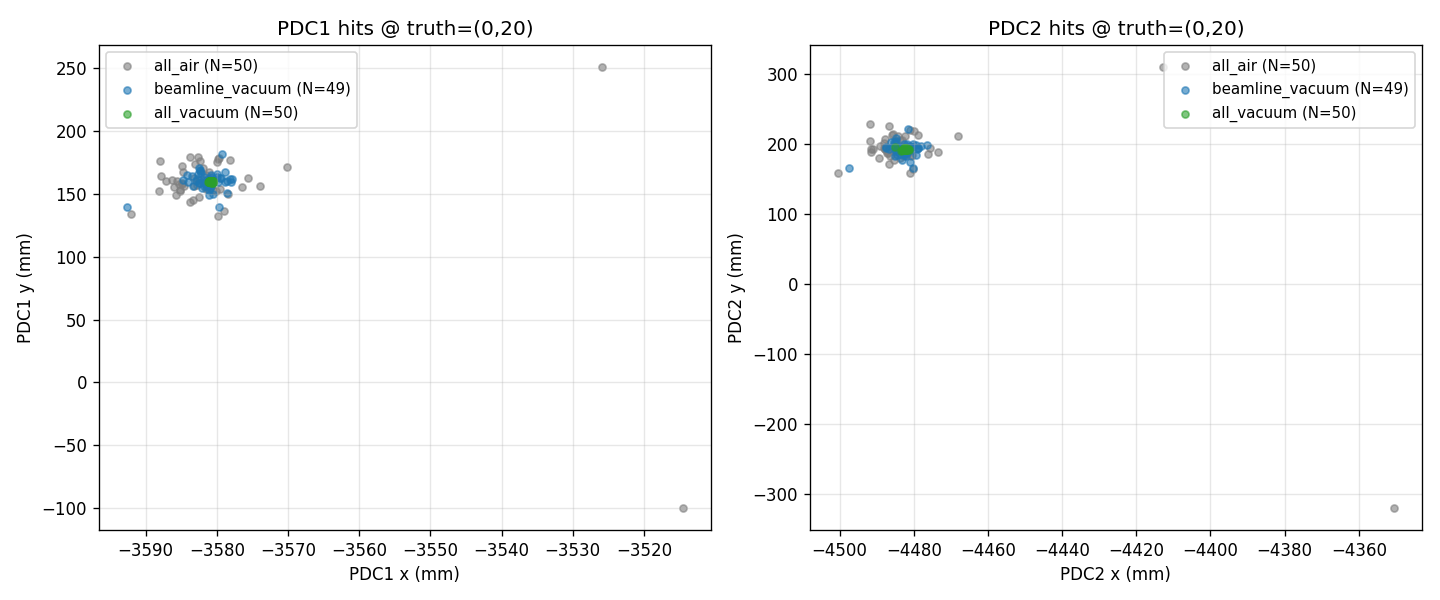
\includegraphics[width=\linewidth]{figures/dispersion_overlay_tp0_20.png}
  \caption{TP3: $(p_x,p_y)=(0,20)$}
\end{subfigure}
\caption{PDC1/PDC2 hit-position scatter for the three configurations ($N=50$ each). Within each panel, left = PDC1, right = PDC2; horizontal axis $x$ [mm], vertical axis $y$ [mm]. Three colours: \texttt{all\_air} (grey), \texttt{beamline\_vacuum} (blue), \texttt{all\_vacuum} (green).}
\label{fig:overlays}
\end{figure}

% ============================================================
\section{Decomposing the two-region air contribution}
% ============================================================

\subsection{Linear differences}

\begin{table}[H]
\centering
\caption{Linear differences in $\sigma_y(\mathrm{PDC2})$ (mm).}
\label{tab:delta_linear}
\begin{tabular}{llrrrr}
\toprule
Difference & Path segment & TP1 & TP2 & TP3 & 3-pt mean \\
\midrule
\texttt{all\_air} $-$ \texttt{beamline\_vacuum}    & Region~A ($\sim 4.3$~m) & 6.025 & 4.540 & 7.468 & \textbf{6.011} \\
\texttt{beamline\_vacuum} $-$ \texttt{all\_vacuum} & Region~B ($\sim 2.0$~m) & 5.854 & 7.213 & 6.456 & \textbf{6.508} \\
\texttt{all\_air} $-$ \texttt{all\_vacuum}         & Full air                & 11.879 & 11.752 & 13.925 & \textbf{12.519} \\
\bottomrule
\end{tabular}
\end{table}

The Region~A and Region~B air contributions to $\sigma_y(\mathrm{PDC2})$ are comparable in magnitude (linear ratio $6.01 : 6.51 \approx 0.92$). Although Region~A's path is more than $2\times$ longer than Region~B's, their contributions are similar because the lever arm projecting Region~A's MS onto the PDC plane (the straight-line drift downstream of the magnet) is shorter than Region~B's --- in Region~B, the MS happens much closer to the PDCs, so its deflection projects with a larger geometric amplification.

\subsection{Quadrature decomposition}

\[
   \sigma_{A} \equiv \sqrt{\sigma_{\mathtt{all\_air}}^{2} - \sigma_{\mathtt{bv}}^{2}}, \qquad
   \sigma_{B} \equiv \sqrt{\sigma_{\mathtt{bv}}^{2}     - \sigma_{\mathtt{av}}^{2}}.
\]

\begin{table}[H]
\centering
\caption{Quadrature decomposition of $\sigma_y(\mathrm{PDC2})$ (mm). The last two columns verify that $\sqrt{\sigma_A^{2}+\sigma_B^{2}+\sigma_{\mathtt{av}}^2}$ recovers the measured \texttt{all\_air} value.}
\label{tab:delta_quadrature}
\begin{tabular}{lrrrr}
\toprule
Truth & $\sigma_A$ (Region~A) & $\sigma_B$ (Region~B) & $\sqrt{\sigma_A^{2}+\sigma_B^{2}+\sigma_{\mathtt{av}}^2}$ & $\sigma_{\mathtt{all\_air}}$ measured \\
\midrule
$(0,0)$   & 10.874 & 6.735 & 12.826 & 12.826 \\
$(100,0)$ &  9.755 & 8.150 & 12.751 & 12.751 \\
$(0,20)$  & 12.930 & 7.391 & 14.927 & 14.927 \\
\midrule
\textbf{3-pt mean} & \textbf{11.19} & \textbf{7.43} & --- & --- \\
\bottomrule
\end{tabular}
\end{table}

The quadrature sum reproduces the measured \texttt{all\_air} value to floating-point precision (residual $< 10^{-3}$~mm) on all three truth points: the assumption ``independent noise sources, $\sigma$'s add in quadrature'' is exactly self-consistent on this dataset.

% ============================================================
\section{Process-noise input for the RK reconstructor}
% ============================================================

The downstream RK reconstruction (stage~D) needs ``the MS-induced $\sigma$ at PDC2 for the chosen experimental configuration''. Depending on whether Region~A is going to be evacuated or kept as air in the experiment, two reference values (3-truth-point mean) are tabulated below:

\begin{center}
\begin{tabular}{lcc}
\toprule
Experimental configuration (Region~A state) & $\sigma_{y,\mathrm{MS}}$(PDC2) & $\sigma_{x,\mathrm{MS}}$(PDC2) \\
\midrule
A = air (no evacuation), B = air      & 13.50 mm & 4.37 mm \\
A = vacuum (evacuated), B = air       &  7.49 mm & 2.50 mm \\
\bottomrule
\end{tabular}
\end{center}

These values are the measured $\sigma$'s of \texttt{all\_air} and \texttt{beamline\_vacuum} directly (the residual instrumental term $\sim 1$~mm from \texttt{all\_vacuum} is small enough to ignore). Per-truth-point breakdown, Region~A evacuated: $\sigma_y(\mathrm{PDC2}) = \{6.80,\ 8.21,\ 7.46\}$~mm. The stage~D spec should cite the numbers from this memo.

% ============================================================
\section{Risks and clarifications}
% ============================================================

\begin{itemize}[nosep]
  \item \textbf{$\sigma$ definition}: throughout, robust half-width $(p_{84}-p_{16})/2$. Equal to RMS for a pure Gaussian; conservative by $\sim 10\%$ on heavy-tailed distributions.
  \item \textbf{TP3 \texttt{beamline\_vacuum} $N=49$}: one event's proton failed to match both PDC planes and was naturally excluded by hit matching ($2\%$ loss).
  \item \textbf{\texttt{all\_vacuum} residual $\sigma_y \sim 1.0$~mm}: comes from PDC gas, ExitWindow flange (currently a 30~mm iron flange, not a thin window) and miscellaneous geometry detail; not a target of the decomposition in this memo.
  \item \textbf{Curvature corrections}: the 4.3~m for Region~A is along the proton's curved trajectory; the straight-line approximation differs from the actual arc length by $< 10\%$. We did not validate against Highland (the changing arc length and $\beta$ make a simple $L/X_0$ formula imprecise); the quadrature decomposition is taken directly from the measured $\sigma$'s.
  \item \textbf{Target off}: all three configurations use \texttt{SetTarget false}, so the proton starts at the target centre.
  \item \textbf{Experimental configuration}: whether Region~A will be air or vacuum in the actual experiment is still being discussed; the three configurations here are ablations and are not endorsements of any particular experimental setup.
\end{itemize}

% ============================================================
\section{Artefact list}
% ============================================================

\begin{itemize}[nosep]
  \item Scripts: \verb|scripts/analysis/ms_ablation/{run_ablation.sh, compute_metrics.py, compare_ablation.py}|
  \item Unit tests: \verb|scripts/analysis/ms_ablation/tests/| (6 tests pass)
  \item Macros: \verb|configs/simulation/DbeamTest/detailMag1to1.2T/|\\
        \verb|geometry_B115T_pdcOptimized_20260227_target3deg{,_mixed,_noair}.mac|
  \item Data snapshot: \verb|docs/reports/reconstruction/momentum_reco/ms_ablation/data/|\\
        \verb|{all_air,beamline_vacuum,all_vacuum}_dispersion_summary.csv|, \verb|compare.csv|
  \item Figures: \verb|docs/reports/reconstruction/momentum_reco/ms_ablation/figures/dispersion_overlay_tp*.png|
\end{itemize}

\textbf{Companion document}: \texttt{ms\_ablation\_mixed\_20260422\_zh.pdf} (Chinese version, identical content).

\end{document}
